\documentclass[10pt,peerreviewca,onecolumn]{IEEEtran} % [11pt,english]{article}
\usepackage{mhchem}
\usepackage{siunitx}
\usepackage{physics}
\usepackage{amsmath}
\usepackage{cuted}
\usepackage{graphicx}
\graphicspath{ {images/} }

\newcommand{\e}{\mathrm{e}}
\newcommand\numberthis{\addtocounter{equation}{1}\tag{\theequation}}
\newcommand{\opmat}[1]{\mathbf{#1}}

\author{
	Lee, Seungsup
	\and
	Miller, Dory
	\and
	Payant, Andrew
	\and
	Powers-Luhn, Justin
	\and
	Zhang, Fan
}

\title{Nuclear Reactor Theory Project \#1\\Group \#3}


\begin{document}
	\pagenumbering{gobble}
	\maketitle
	\newpage
	\pagenumbering{arabic}

	\begin{abstract}
		THIS IS THE ABSTRACT
	\end{abstract}
	
	\section{Introduction \& Background}
	Proving the capabilities and safety of a reactor design requires effective modeling of the neutron flux in the core (expressed in equation \ref{eqn:transport}). For real cores, however, this is impossible, and must be first simplified, then discretized to provide the solution for a representative mesh. 

	For this project we have analyzed a simplified, monoenergetic, non-multiplying medium in one dimension. The flux originates from a single source at $x=0$ with a strength of $S=\SI{1E8}{\per\second}$. These assumptions simplify the transport equation to that presented in equation \ref{eqn:simplified_diffusion}.

	In the following sections, we will first describe the terms in equation \ref{eqn:simplified_diffusion}, then provide both an analytical and a discrete solution. We will also provide an analysis of the accuracy of the analysis as a function of the number of nodes. Finally, we will analzye the solution for different coordinate systems to equation \ref{eqn:simplified_diffusion}.

	%\begin{strip}
	\begin{equation}
		\pdv{n}{t} + v \hat{\Omega} \cdot \nabla n + v \Sigma_t n \left( \mathbf{r}, E^\prime, \hat{\Omega}, t \right) = \\ \int_{4\pi} d \hat{\Omega} ^\prime \int_0^{\infty} dE ^\prime v^\prime \Sigma_s\left( E ^\prime \rightarrow E, \hat{\Omega} ^\prime \rightarrow \hat{\Omega} \right) n\left( \mathbf{r}, E ^\prime, \hat{\Omega} ^\prime, t \right) + s\left( \mathbf{r}, E, \hat{\Omega}, t \right)
		\label{eqn:transport}
	\end{equation}
	%\end{strip}

	\begin{equation}
		-D_m \dv[2]{\phi}{x} + \Sigma^m_a \phi = 
		\begin{cases}
			S & \left(x=0\right) \\
			0 & \left(x>0\right)
		\end{cases}
		\label{eqn:simplified_diffusion}
	\end{equation}

	\begin{table*}
		\begin{center}
		\begin{tabular}{ c c c c c }
			\hline
			\textit{Material} & $ \Sigma_{tr}(\si{cm^{-1}}) $ & $ \Sigma_a (\si{cm^{-1}}) $ & $ \nu \Sigma_f (\si{cm^{-1}}) $ & \textit{Relative Absorption} \\
			\hline
			\ce{H} & \num{1.79e-2} & \num{8.08e-3} & 0 & \num{0.053} \\
			\ce{O} & \num{7.16e-3} & \num{4.90e-6} & \num{0} & \num{0}\\
			\ce{Zr} & \num{2.91e-3} & \num{7.01e-4} & \num{0} & \num{0.005} \\
			\ce{Fe} & \num{9.46e-4} & \num{3.99e-3} & \num{0} & \num{0.026} \\
			\ce{^{235}U} & \num{3.08e-4} & \num{9.24e-2} & \num{0.145} & \num{0.602} \\
			\ce{^{238}U} &\num{6.95e-3} & \num{1.39e-2} & \num{1.20e-2} & \num{0.091} \\
			\ce{^{10}B} & \num{8.77e-6} & \num{3.41e-2} & \num{0} & \num{0.223} \\
			\hline
			& \num{3.62e-2} & \num{0.1532} & \num{0.1570} & \num{1.000} \\
			\hline
		\end{tabular}
		\label{materials_table}
		\caption{Macroscopic Cross Sections}
		\end{center}
	\end{table*}

	\section{Methodology}
	Equation \ref{eqn:simplified_diffusion} is a simplified description of neutron diffusion through a finite medium, similar to a point source travelling through a shielding material to a detector. The flux, therefore, depends on the transport cross section. This is accounted for in the term $D_m$, which is related to the transport coefficient by $D_m = 3 \Sigma_{tr}^{-1}$. Values for $\Sigma_{tr}$ for typical reactor materials are found in table \ref{materials_table}. 

	\subsection{Analytic Solution}
	In the slab, equation \ref{eqn:simplified_diffusion} is equal to $0$, $-D_m \pdv[2]{\phi}{x} + \Sigma^m_a \phi = 0 $. In order to better group constants, specify a diffusion length, $L = \sqrt{D_m / \Sigma_{a}}$. We can then solve for $\phi(x)$:
	\begin{align*}
		\pdv[2]{\phi}{x} - \frac{\phi}{L} &= 0 \\
		\phi(x) &= A \e^{-x/L} + C \e^{x/L} \numberthis \label{eqn:generalsolution}
	\end{align*}
	First use the boundary condition $\phi(w)=0$ to solve for $C$
	\begin{align*}
		0 &= A \e^{-w/L} + C \e^{w/L} \\
		C &= -A \e^{2w/L} \\
	\end{align*}
	Next, use the fact that $ -D_m \phi^\prime(0) = J(0) = S/2$ to solve for $A$
	\begin{align*}
		J(0) = \frac{S}{2} &= -\frac{A}{L} \left( 1 + \e^{-2w/L} \right) \\
		A &= \frac{S L}{2 D_m}\left( 1 + \e^{-2w/L} \right)^{-1}
	\end{align*}
	Substituting this in to equation \ref{eqn:generalsolution}, we get:
	\begin{equation*}
		\phi(x) = \frac{S L}{2 D_m} \left( \frac{\e^{-x/L} - \e^{\left(x-2w\right)/L}}{1 - \e^{-2w/L}} \right) \numberthis \label{eqn:analyticcartesian}
	\end{equation*}

	\subsection{Numerical Approximation}
	It is rare to be faced with a design that allows for an analytical solution. Fortunately, numerical analysis methods exist that allow for approximation of the analytical solution. By dividing our hypothetical medium into discrete sections with nodes at the boundaries between these sections, it is possible to express the flux vector with equation \ref{eqn:linalg_flux}.

	\begin{equation}
		\opmat{A} \vec{\phi} = \vec{S}
		\label{eqn:linalg_flux}
	\end{equation}
	
	\section{Results}
	\begin{figure}[h]
		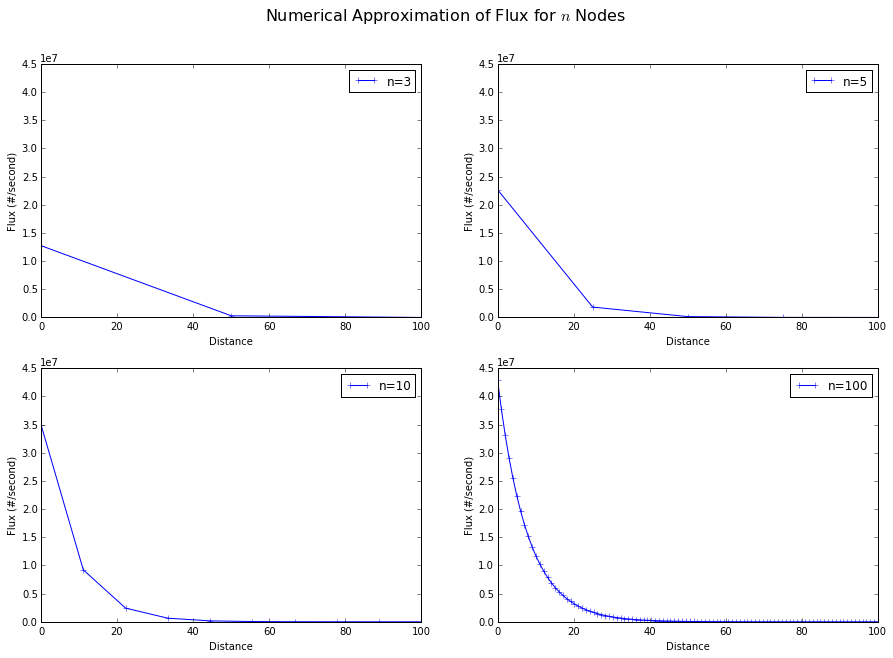
\includegraphics[width=7in]{curve_vs_number_of_nodes}
		\caption{Numerical Solution for 3, 5, 10, and 100 Nodes}
		\label{fig:numnodes}
	\end{figure}

	\begin{figure}[h]
		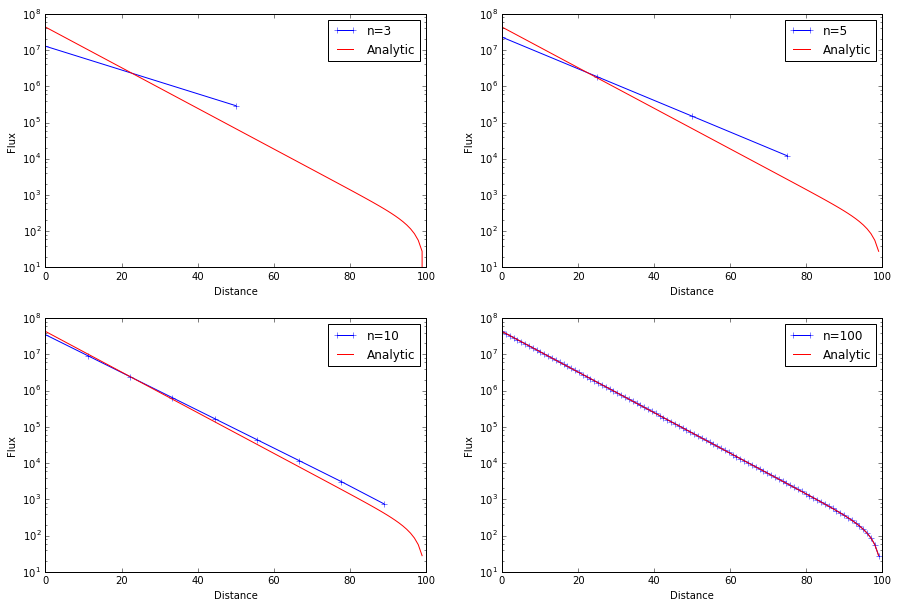
\includegraphics[width=7in]{analytic_vs_numerical}
		\caption{Comparison of Numerical and Analytical Solutions}
		\label{fig:numerical_vs_analytical}
	\end{figure}
	
	\section{Conclusions}
	The conclusions go here



\end{document}
